\documentclass[fontset=windows,a4paper,12pt]{ctexart}
\usepackage{geometry}
\usepackage{graphicx}
\usepackage{subfigure}
\usepackage{graphics}
%\usepackage{overcite}
\usepackage{url}
\usepackage{listings}
\usepackage{CJK}
\usepackage{booktabs} 
\pagestyle{plain}
\usepackage{bm}
\usepackage{amsmath}
\usepackage{multirow}

\geometry{top=25.4mm,bottom=25.4mm,left=31.75mm,right=31.75mm}
\newcommand{\upcite}[1]{\textsuperscript{\textsuperscript{\cite{#1}}}}
\renewcommand{\eqref}[1]{公式 (\ref{#1})}
\renewcommand*{\baselinestretch}{1.38}

\begin{document}
  \begin{center}
  	\zihao{3}{\heiti 小区开放对道路通行的影响}
  \end{center}
  \linespread{1.2}
  \begin{center}
  	\zihao{4}{\heiti 摘\ \ \ \ 要}
  \end{center}
  \zihao{4}{\songti 
  	\quad \quad 本文对小区开放问题产生的影响进行研究,以考察小区开放对路网优化、道路通行能力提升、交通状况改善的效果为主要目标,从道路结构、交通流量、人为因素等角度出发,对不同影响因素逐一分析并建立相应的数学模型,定量分析小区开放对周边道路通行的影响。
  	
  	对于问题一,通过对国内外开放小区与封闭型小区的对比,分析小区开放对周边道路产生的影响,建立影响因素与道路、交通条件的关系,进而确定小区开放对周边道路的影响因素,即路网变化、行人等非机动车、新增路口三个因素会对周边道路通行产生影响。通过构建模糊综合评价模型,建立各影响因素对周边道路通行影响程度的关系矩阵,构建评价指标体系。

	对于问题二,根据评价指标模型中小区开放对周边道路通行的影响因素,考虑车辆通行过程中所需时间、交通需求和交通流量分配三个因素,建立车辆通行的数学模型,以研究小区开放对周边道路通行的影响。其中车辆通行所需总时间可由延误时间和行驶时间构成,利用基于breass悖论判别系统,判别交通需求的变化是否产生breass悖论现象。通过动态交通分配分析最优的交通流量分布模式,并对交通需求进行合理配置。                 

	对于问题三,构建三种不同类型的小区,综合问题一中的评价模型,建立元胞自动机模型对三种不同类型的小区进行仿真模拟,以真实可靠的数据结果验证该类型小区是否适合开放及开放后产生的影响。

	最后,通过对小区开放影响的研究,就小区开放前后对周边影响程度,结合评价指标,向城市规划和交通管理部门提出小区开放的建议,以实现小区开放后路网结构得以优化、道路通行能力提高、交通状况改善的目的。

  }
  \textbf{关键词:}\ 模糊评价\ BPR函数
  \newpage
  \section{问题重述}
	基于“适用、经济、绿色、美观”的理念,为塑造城市良好风貌,缓解城市交通压力,促进土地节约利用,实现内部道路公共化,实现城市有序建设、适度开发、高效运行,近来,国务院发布的《关于进一步加强城市规划建设管理工作的若干意见》中指出,原则上不允许再建设封闭式小区,已建成的单位大院和住宅小区要逐步实现开放。此政策的颁布,引起了广泛的关注和讨论。

	然而小区由封闭型转向开放型,并非只拆除外部围墙就能达到。小区开放,即外部车辆可自由进出小区,小区内部道路作为市政道路使用。对此,大家产生疑惑:小区开放能否达到道路网结构优化,提高道路通行能力,改善交通状况的目的。如果小区开放能对周边道路通行能力起到改善效果,那么改善效果如何?对此,产生四种不同的观点:第一种观点认为,封闭型小区土地使用效率低,对土地分块化,破坏城市路网结构,堵塞路网结构中的“毛细血管”,增大路网压力,容易造成交通阻塞,不利于实现城市有序、高效建设的目标;第二种观点认为,小区开放增加了路网中道路数目,即路网密度增大,道路面积增加,通行能力自然有所提升;第三种观点认为,道路通行能力与小区位置、面积、内外部道路状况等诸多因素有关,不能一概而论小区开放产生的影响;还有一种观点认为,小区开放可以增加道路数量,但与此同时小区周边主路上进出小区交叉路口的车辆也相应的增加,可能会对主路的通行速度产生消极影响。

	现需要就小区开放对周边道路通行的影响进行研究,建立适当的数学模型并做定量分析,解决以下四个问题:
\begin{enumerate}
	\item 构建评价小区开放对周边道路通行影响的评价指标体系。
	\item 建立与车辆通行与路网相关的数学模型以研究小区开放对周边道路通行的影响。
	\item 小区结构及周边道路的车流量、道路结构可能会对小区开放效果产生影响。选取或构建不同类型的小区,运用上述过程中所建立的模型,就各类型小区开放前后对道路通行的影响进行比较并作定量分析。
	\item 根据上述研究结果,从交通通行的角度,向城市规划和交通管理部门提出关于小区开放的合理化建议。
\end{enumerate}
  \section{符号说明}
  \begin{tabular}{c|c}
	\toprule[1pt]
	\makebox[0.4\textwidth][c]{符号}	&  \makebox[0.5\textwidth][c]{意义} \\ \hline
	U				&	影响因素集\\
	V				&	评判等级集\\
	T				&	行程时间\\
	$G(N,L)$		&	交通网络\\
	$q_a$			&	路段a上的流量\\
	$Q_p$			&	路径p上的流量\\
	$r_a$			&	路段a上的阻抗\\
	$R_a$			&	路径p上的阻抗\\
	$\eta,\eta_b$	&	行人与非机动车影响系数\\
	\bottomrule[1pt]
\end{tabular}
  \section{问题分析}
  随着经济的发展,道路压力越来越大,我国现行的路网结构无法满足日益增长的车流量需求,而国外的小区开放制度对交通压力的缓解方式值得借鉴。根据对国内外开放小区与封闭小区数据的收集和对比,得到表\ref{tab:net_density}中的数据。
  \begin{table}[!htbp]
	\centering
	\caption{国际城市与国内城市路网密度对比\upcite{国外街区制是如何完美炼成}}
	\label{tab:net_density}
	\begin{tabular}{cc|cc}
		\toprule[1pt]
		国内城市 & 路网密度($km/km^2$) & 国际城市 & 路网密度($km/km^2$) \\ 
		\hline%\midrule[1pt]
		北京 & 6.3 & 芝加哥 & 18.6 \\ 
		上海 & 6.7 & 纽约 & 13.1 \\ 
		深圳 & 5.7 & 东京 & 18.4 \\ 
		武汉 & 9.8 & 大阪 & 18.1 \\ 
		大连 & 6.0 & 横滨 & 19.2 \\ 
		成都 & 5.9 & 巴塞罗那 & 11.2 \\ 
		杭州 & 5.2 &  &  \\ 
		昆明 & 4.7 &  &  \\ 
		\bottomrule[1pt]
	\end{tabular} 
  \end{table}
  
  由表\ref{tab:net_density}中的数据,容易得到我国城市当今的道路密度远低于国际其他城市。而这种差距在地图上看来更为直观,如图\ref{fig:cmp_tokyo_beijing}中(a)为北京的路网密度(b)为东京路网密度。
  \begin{figure}[!htbp]
  	 \centering
	 \subfigure[北京东二环]{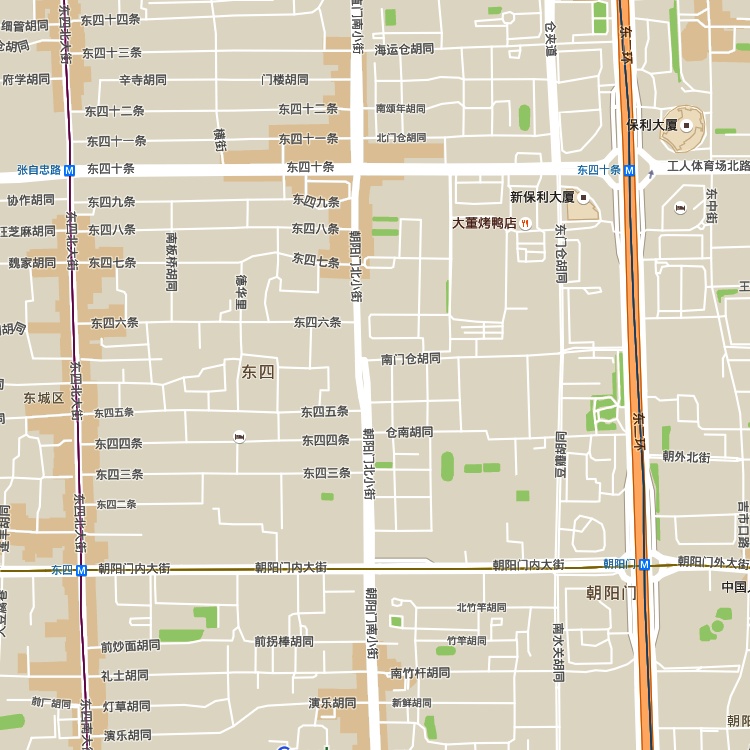
\includegraphics[width=0.4\textwidth]{pic/beijing.png}}
	 \subfigure[东京千代田区]{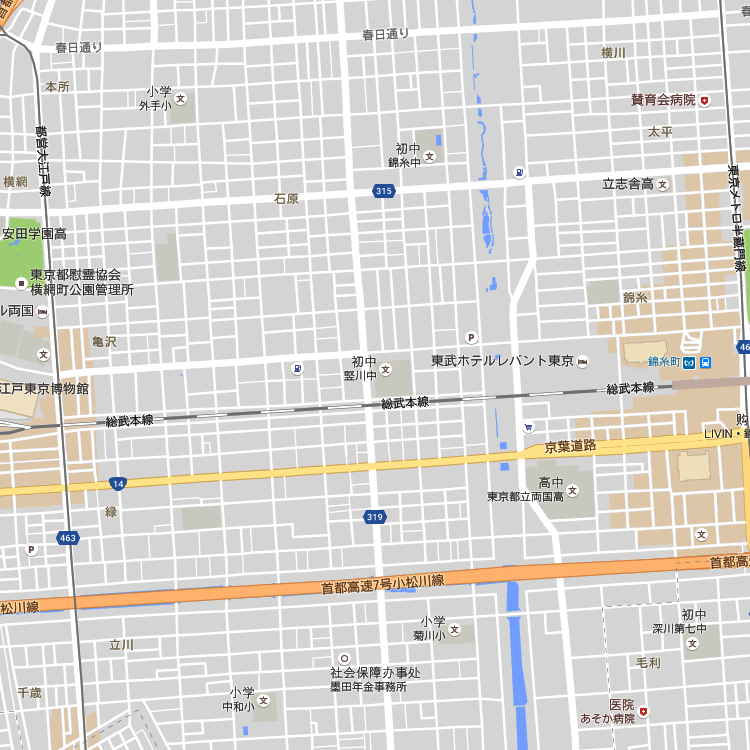
\includegraphics[width=0.4\textwidth]{pic/tokyo.png}}
	 \caption{同高度下北京与东京的路网密度对比}
	 \label{fig:cmp_tokyo_beijing}
  \end{figure}
  因此增加我国城市的路网密度是缓解交通压力的必要选择,而实行小区开放政策能否对周边道路的通行产生积极影响有待考究。本文通过对小区开放后产生的变化进行分析,就路网结构、新增道路口、人流量和非机动车流量对道路通行的影响进行分析,研究小区开放产生的影响。
  
	针对问题一,要建立评价指标体系,则需考虑小区开放对周边道路通行的影响因素,并通过各影响因素特性和各因素之间联系构建评价指标。通过对国内外开放小区与封闭型小区的对比,分析小区开放对周边道路通行的影响因素,考虑路网变化、行人等非机动车、新增路口三个因素,并建立影响因素之间的关系。通过构建模糊综合评价模型,建立各影响因素对周边道路通行影响程度的关系矩阵,构建评价指标体系。
	
	针对问题二,根据问题一中评价指标模型中小区开放对的影响因素,建立相应的数学模型,研究小区开放的影响。道路通行能力受多重因素的影响,车辆通行与多方面参量有关,考虑车辆通行过程中交通阻抗、交通流量和交通流量分配三个因素,建立车辆通行的数学模型,以研究小区开放对周边道路通行的影响。利用基于breass悖论的判别系统判别小区开放后的交通流量是否出现breass悖论现象。由于道路数目增加,可能造成Breass悖论的出现,故增加道路数目需满足不产生Breass悖论现象,根据判别系统,求解出不产生Breass悖论所满足的交通需求。当小区开放满足所需时间最短、交通流量分配最佳且所增加道路数不出现breass悖论时,该小区适合开放,且开放小区对周边道路产生积极影响;否则,该小区开放在一定程度上会对周边道路通行产生消极影响。  
	
	针对问题三,搜集不同小区的数据,构建三种不同类型的小区,综合问题一中的评价模型,通过建立元胞自动机模型对上述三种不同类型的小区进行仿真模拟,结果结合问题一中评价指标,考究该类型小区是否适合开放及开放后产生的影响。
	
	针对问题四,通过对以上问题的研究,对小区开放的影响产生一定的理解和认识,基于文中的研究内容,向城市规划和交通管理部门提出小区开放的建议,以实现小区开放后路网结构得以优化、道路通行能力提高、交通状况改善的目的。
  \section{模型建立}
	  
	\subsection{问题一}
		根据对开放小区与封闭型小区进行对比、分析,得到小区开放会引起众多因素的变化,如:道路网结构的改变、机动车受行人与非机动车的影响和道路口的增加。小区开放后,车辆可自由出入小区,小区内部道路转变为市政道路,引起现有道路网中道路数目的变化;小区内行人、自行车等非机动车较多,在实际通行中不免产生行人、非机动车对机动车通行的影响,为简化模型、省去不必要的因素,不妨假设用自行车对机动车的影响代替非机动车对机动车的影响;小区路段开放后与市政道路衔接处产生路口,而路口处是整条路上交通压力最大的地方,因而不可忽略新增路口数目的影响。

		
		\subsubsection{模糊评价模型}
			评价指标体系是用来表征各影响因素特性和各因素之间联系的指标,图\ref{fig:layer_struct}构建了影响因素的分层结构。通过建立模糊评价模型,构造评判矩阵,求得评价结果,从而得到评价指标各等级程度。
			\begin{figure}[!htbp]
				\centering
				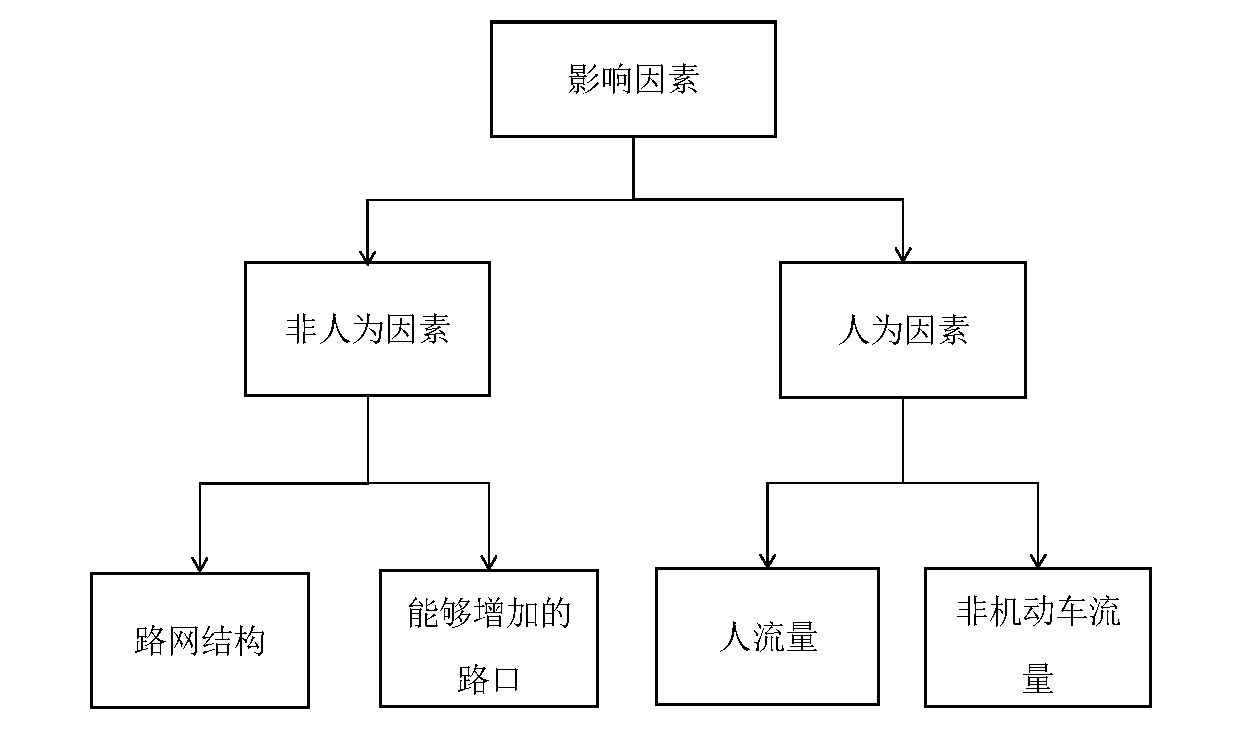
\includegraphics[width=0.7\textwidth]{pic/judge_result.pdf}
				\caption{影响因素的分层次结构}
				\label{fig:layer_struct}
			\end{figure}
			设影响因素的因素集$ U=\{u_1,u_2,u_3\} $,评判等级集$ V=\{v_1,v_2,v_3\} $。
			其中$ U $中$ u_1 $代表路网结构改变对周边道路的影响,$ u_2 $代表人流量与非机动车流量对周边道路的影响,$ u_3 $代表可能增加的路口对周边道路造成的影响;$ V $中$ v_1 $代表开放小区对周边道路交通有积极影响,$ v_2 $代表开放小区对周边道路交通的改善效果一般,$ v_3 $代表开放小区对周边道路交通有不利影响。
			对U中每一个因素根据评判等级指标进行模糊评判,得到评判矩阵为:
			$$
				R=\left[
				\begin{array}{cccc}
					r_{11} & r_{12} & r_{13}\\
					r_{21} & r_{22} & r_{23}\\
					r_{31} & r_{32} & r_{33}
				\end{array}
				\right]
			$$
			其中$ r_{ij} $表示$ u_i $关于$ v_j $的隶属程度,则$ (U,V,R) $构成一个模糊评价模型,利用层次分析的方法确定各项因素的权重,比较影响因素集U中的元素,得到比较矩阵为:
			$$
				C=\left[
				\begin{array}{cccc}
					1 & 5 & 3\\
					1/5 & 1 & 1/2\\
					1/3 & 2 & 1
				\end{array}
				\right]
			$$
			得到C的特征向量$ D=[-0.9281,-0.1747,-0.3288] $,将向量标准化之后为$ D'=[0.6483 0.1220,0.2297]^Z $
			则评价模型中的权重因素记为$A$并且令$ A=D' $,满足$ \sum\limits_{i=1}^{3}a_i=1 $,
			综合评价为:
			\begin{equation}
				\overline{B}=A \cdot R=(\overline{b_1},\overline{b_2},\overline{b_3}) 
				\label{eq:judge_result}
			\end{equation}
			\eqref{eq:judge_result}即是开放小区对周边交通影响的评价结果,其中$\overline{b_1},\overline{b_2},\overline{b_3}$分
			别代表主要因素对于评判等级的隶属度,归一化后我们还可以得到开放小区对周边的影响趋向某一个等级的程度即$ B=(b_1,b_2,b_3) $。

	\subsection{问题二}
		交通网络通行主要受到道路阻抗的影响道,路阻抗是表达车辆在运行过程中受到的阻碍程度的高低的量值,是城市交通网络研究中的重要参量,它直接影响交通流的路径选择和流量分配。
		
		在一个交通网络$G(N,L)$中,N为网络中的节点集合,L为网络中的路段集合。现有出发地/目的地(OD)的集合W含有$n_w$个元素,链接W中路径的集合记为$P$,链接P中每个元素的路径的集合记为$P_w$,记$t_a$为路段a的行程时间,$r_a$为路段a上的阻抗,$R_p$记为路径p上的阻抗,$T_p$为路径p的行程时间,$q_a$为路段a的流量,$Q_p$为路径p上的流量,$d_w$记为P中路径的交通需求,根据以上条件建立模型\upcite{赵春雪2012拥挤交通网络的}。
		
		一般情况下,某一路段的在某一时刻的阻抗$r$不仅与本路段流量有关还与其他路段的交通流量有关,在此,为了简化模型,我们假设本路段流量只与自身流量和与之相邻路段的流量有关,如\eqref{eq:res_for_a}所示,其中$\{1,2,\dots,\varPhi\}$为与a在同一路径的路段集合。
		\begin{equation}
			r_a=r_a(q_a,q_1,q_2,\dots,q_\varPhi),\quad\forall a \in L
			\label{eq:res_for_a}
		\end{equation}
		某一路径p上的流量可以由该路径上路段的流量的加和表示,其关系可以表示为\eqref{eq:qud_for_a},其中如果路段a在路径p上,那么$k_ap=1$否则为0。
		\begin{equation}
			Q_a=\sum\limits_{a\in L}q_ak_ap,\quad\forall a \in L
			\label{eq:qud_for_a}
		\end{equation}
		由\eqref{eq:res_for_a}和\eqref{eq:qud_for_a}可以得阻抗到在某一路径p上的表达式如\eqref{eq:res_for_p}所示,其中$\{1,2,\dots,\Lambda\}$,为包含a或与a相邻的路径集合。
		
		\begin{equation}
			R_a=\sum\limits_{p\in P}r_a(q_a,q_1,q_2,\dots,q_\Lambda)k_ap,\quad\forall p \in P
			\label{eq:res_for_p}
		\end{equation}
		
		车辆在某一路段受到的阻抗可以分为在某一路段上的阻抗,与因为其他因素造成的延误的阻抗,所以车辆经过一段路程的总阻抗可以由\eqref{eq:time_total}表示,其中$ t_d $为延误造成的阻抗,$t(q)$为由路阻函数得到的阻抗。
		\begin{equation}
			r = t_d + t(q)
			\label{eq:time_total}
		\end{equation}		
		
		\subsubsection{延误时间造成的阻抗}
			延误时间\upcite{任福田2003交通工程学}是指,道路上通行所需时间除行走时间外,也受市政道路交通信号灯的影响,如\eqref{eq:delay_func}所示。
			\begin{equation}
				t_d=\frac{0.5T(1-\frac{t_g}{T})}{1-[min(1,v/c)\cdot{\frac{t_g}{T}}]}
				\label{eq:delay_func}
			\end{equation}
			其中$ T $表示信号灯周期长度,$ t_g $代表绿灯时间,$ v,c $代表最大交通量与基本交通量。
			
			并且,开放小区后必然会增加某些路口,而开放新的的路口又会增大道路的延误时间,因此为了了解开放路口对周边道路的影响,我们需要对支路与街区道路的接口进行分析,对于最终对周边道路的影响我们使用Vissim软件进行仿真模拟。
		\subsubsection{改进道路阻抗模型}
					
			目前广泛使用的路阻函数是美国联邦公路局路阻函数(即BPR函数)如\eqref{eq:bpr_plain}所示。
			\begin{equation}
				t(q)=t_0(1+\alpha(q/c)^\beta)
				\label{eq:bpr_plain}
			\end{equation}
			其中$ t(q) $表示流量为q时该路段的行程时间,$ t_0 $为该路段的自由流行程时间,$ c $为该路段上的实际通行能力,$ \alpha,\beta $为回归系数,一般取$ \alpha=0.15,\beta=4 $由于模型中的c并不具有固定的含义\upcite{郑远2007美国联邦公路局路阻函数探讨},在实践过程中使用BPR函数的效果并不理想,查阅论文我们采取修正过的BPR函数,并且考虑到小区内道路上行人、自行车等非机动车较多的
			特点,增加行人对机动车的影响、自行车对机动车的影响对其改进,结合已有的研究成果\upcite{李向朋2014城市交通拥堵对策—封闭型小区交通开放研究},得到行人干扰修正系数如表\ref{tab:walker_noise}。
			
			\begin{table}[!htbp]
				\centering
				\caption{行人干扰的修正系数}
				\label{tab:walker_noise}
				\begin{tabular}{c|cccccc}
					\toprule[1pt]
					干扰程度  & 无 & 很小 & 一般 & 较严重 & 严重 & 很严重  \\ 
					\hline 
					$\eta$  & 1.0 & 0.9 & 0.8  & 0.7 & 0.6 & 0.5 \\ 
					\bottomrule[1pt]
				\end{tabular}
			\end{table}
			新开放的小区路线一般为双向两车道的城市支路,车流量的构成十分复杂,具有大量行人与非机动车干扰,当非机动车的流量没有超过道路通行能力时,非机动车对机动车的影响系数取0.8,而当非机动车的流量超过道路通行能力时非机动车对车辆的影响系数由\eqref{eq:bike}得到。Vissim是由德国PTV公司发布的用于交通仿真的仿真软件,广泛用于有关交通系统的模拟之中。
			\begin{equation}
				\eta_b = 0.8-\frac{(q_b/Q_b+0.5-W_2)}{W_1}
				\label{eq:bike}
			\end{equation}
			其中$ \eta_b $非机动车干扰系数,$ q_b $非机动车流量,$ Q_b $非机动车道通行能力$ W_1,W_2 $
			非机动车道宽度与机动车道宽度。
			
			综上所述,得到改进BPR路阻函数如\eqref{eq:bpr_imporve}。
			\begin{equation}
				t(q)=\left\lbrace
				\begin{array}{ll}
					t_0(1+\alpha(\frac{qv}{c\eta\eta_b})^\beta), & 0\leq\eta_b\leq1\\
					t_0(1+\alpha(\frac{\eta_bqv}{c\eta})^\beta), & 1\leq\eta_b
				\end{array}	
				\right.
				\label{eq:bpr_imporve}
			\end{equation}			
			则\eqref{eq:time_total}可以表示为\eqref{eq:time_final}所示形式。
			\begin{equation}
				T=\left\lbrace
				\begin{array}{ll}
					t_0(1+\alpha(\frac{qv}{c\eta\eta_b})^\beta)+\frac{0.5T(1-\frac{t_g}{T})}{1-[min(1,v/c)\cdot{\frac{t_g}{T}}]}, & 0\leq\eta_b\leq1\\
					t_0(1+\alpha(\frac{\eta_bqv}{c\eta})^\beta)+\frac{0.5T(1-\frac{t_g}{T})}{1-[min(1,v/c)\cdot{\frac{t_g}{T}}]}, & 1\leq\eta_b
				\end{array}	
				\right.
				\label{eq:time_final}
			\end{equation}
		\subsubsection{Braess悖论}
			数学家Dietrich Braess在1968年首次提出了Braess悖论\upcite{Braess1968Ü}。
			考虑拓扑结构如图\ref{fig:braess}的交通网,假设交通网中的流量为4000,起点为	A,终点为D
			通过$ A \rightarrow B $与$ C \rightarrow D $的时间均为车流量除以100,	通
			过$ B \rightarrow D $与$ A \rightarrow C $的时间为固定的45分钟。
			\begin{figure}[!htbp]
				\centering
				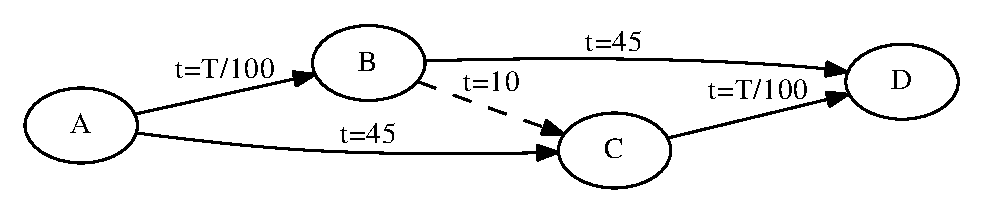
\includegraphics[width=0.5\textwidth]{pic/braess.eps}
				\caption{Braess悖论的具体情况}
				\label{fig:braess}
			\end{figure}
			在路径$ B \rightarrow C $没有开通时,从$ A \rightarrow D $的通过时间分别为$ \frac{A}{100}+45 $与$ \frac{B}
			{100} + 45 $,达到均衡之后有$ A=B=2000 $这样每条路通过的时间都是$ \frac{2000}{100}
			+45=65 $分钟。
		
			现在考虑$ B \rightarrow C $开通之后,其通过时间非常短,在这种情况下,所有司机都会选择$ A \rightarrow B \rightarrow C \rightarrow D $这条路线,因为即使所有车辆全部通过$ A \rightarrow B $所用时间也不超过40分钟,这样所有通过这条路径的时间为$ \frac{4000}{100}\times 2+10=90$分钟,Braess悖论便是指这种情况。		
		\subsubsection{交通分配模型}
			交通分配是指根据现有道路网络,按照一定规则将进入交通网络的流量合理地分配道网络中的各个道路上,并由此得到网络中各个路段的数据,每种不同的规则对应着不同的分配方法\upcite{陆化普1996动态交通分配理论的回顾与展望}。
			下面对比两种重要的交通分配模型:用户平衡与系统最优\upcite{陆化普2006交通规划理论与方法}。
			
			在用户平衡分配中,交通网络中的每个个体都会选择使自己出行时间最短的路径,其数学表达式如\eqref{eq:ue_equation}所示,其中$Q^*$为交通流,$\lambda_w$为最小交通阻抗。
			\begin{equation}
				\begin{array}{c}
					\hat{R_p}(Q^*)=\lambda_w,\quad Q_p^* > 0\\
					\hat{R_p}(Q^*)\leq\lambda_w,\quad Q_p^* = 0
				\end{array}
				\label{eq:ue_equation}
			\end{equation}
			
			而系统最优分配的主要目的是使系统分配的总阻抗最小,如所示,其中$\nu_w$为最小边界路径阻抗。
			\begin{equation}
				\begin{array}{c}
					\hat{R_p}(Q^*)=\nu_w,\quad Q_p^* > 0\\
					\hat{R_p}(Q^*)\leq\nu_w,\quad Q_p^* = 0
				\end{array}
				\label{eq:so_equation}
			\end{equation}
			经过查阅文献\upcite{李向朋2014城市交通拥堵对策—封闭型小区交通开放研究}我们选择使用系统最优分配来决定交通网络流量的选择。
		\subsubsection{基于系统最优分配Braess悖论的判别}
			小区开放相当于在原有的交通网络中再次加入新的网络,其中必然会存在某些情况导致Braess悖论的发生,而出现这种情况时不宜开放小区。
			
			查阅论文可知Pas和Principcipio在其论文中指出了Braess悖论不发生的两种情况\upcite{pas1997braess},一种是交通需求量低时,如\eqref{eq:Q_low},另一种时交通需求量高时\eqref{eq:Q_high},当交通量符合上述两种情况时,不发生Braess现象,其中$\alpha_n$与$\beta_n$分别为总阻抗函数的常数项系数与一次项系数。
			\begin{equation}
				Q<\frac{2(\alpha_1-\alpha_2)}{3\beta_1+\beta_2}
				\label{eq:Q_low}
			\end{equation}
			\begin{equation}
				Q>\frac{2(\alpha_1-\alpha_2)}{\beta_1-\beta_2}
				\label{eq:Q_high}
			\end{equation}
	\subsection{问题三}
		在城市交通中,交通网络通行能力的大小会受到一路段或某一路口的影响于,一般道路等级高的路段会有更多的容纳能力,根据《城市道路工程设计规范》我国城市公路分级如表\ref{tab:road_type}所示。
		\begin{table}[!htbp]
			\centering
			\caption{公路等级类型表}
			\label{tab:road_type}
			\begin{tabular}{c|ccc}
				\toprule[1pt]
				项目级别&设计车速(km/h)&单向机动车道数(条)&分隔带设置\\
				\hline
				快速路	&60-100	&$\geq$4	&必须设\\
				主干路	&60-40	&$\geq$4	&应设\\
				次干路	&30-50	&$\geq$2	&可设\\
				支路	 &20-40	 &2			&不设\\
				\bottomrule[1pt]
			\end{tabular}
		\end{table}
		
		市区街道大多属于主干路与次干路,而封闭式小区中大多为支路等级的道路,由此我们构建了三种不同类型的小区如表\ref{tab:apartment_type}所示。
		\begin{table}[!htbp]
			\centering
			\caption{小区类型表}
			\label{tab:apartment_type}
			\begin{tabular}{c|cccc}
				\toprule[1pt] 
				类型 & 道路等级 & 周围道路等级 & 人车分离 & 出口数量 \\ 
				\hline 
				A型 & 支路 & 次干道 & 不分离 &  5\\ 
				B型 & 支路 & 次干道 &  分离&  3\\ 
				C型 & 支路 & 主干路 &  分离&  4\\ 
				\bottomrule[1pt]
				\end{tabular} 
		\end{table}
		\begin{figure}[!htbp]
			\centering
			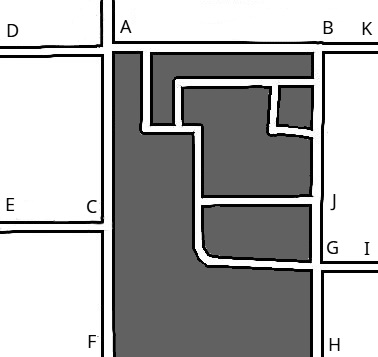
\includegraphics[width=0.5\textwidth]{pic/net_a.jpg}
			\caption{A类型小区的路网结构}
			\label{fig:net_a}
		\end{figure}		
		首先考虑A类型小区如图\ref{fig:net_a}所示,其中灰色区域为原封闭小区区域,周围道路设施情况如表\ref{tab:road_level_a}所示。

		\begin{table}[!htbp]
			\centering
			\caption{A型小区道路等级表}
			\label{tab:road_level_a}
			\begin{tabular}{c|ccc}
				\toprule[1pt] 
				道路&				道路等级&	车道数量&	人车分离\\
				\hline
				D-K&	主干道&	4&			分离\\
				A-F&	主干道&	4&			分离\\
				E-C&	次干道&	2&			不分离\\
				G-I&	次干道&	2&			不分离\\
				B-H&	主干道&	4&			分离\\
				其余小区内道路	&	支路&		2&			不分离\\
				\bottomrule[1pt]
			\end{tabular} 
		\end{table}
		图中每条路段上的车流量我们通过Vissim模拟得到如表\ref{tab:car_flow_a}所示。
		\begin{table}[!htbp]
			\centering
			\caption{路口机动车流量表}
			\label{tab:car_flow_a}
			\begin{tabular}{c|ccccccccc}
				\toprule[1pt] 
				路段&	D-A&	G-I&	B-G&	G-H&	A-B&	A-C&	C-F&	B-K&	C-E\\
				流量&	4730&	2410&	3870&	4467&	6450&	7310&	4730&	3870&	1875\\
				\bottomrule[1pt]
			\end{tabular} 
		\end{table}
		在我国《城市道路工程设计规范》中给出了车道基本通行能力与设计通行能力值如表\ref{tab:road_flow}所示。
		\begin{table}[!htbp]
			\centering
			\caption{一般等级道路路段一条车道的通行能力}
			\label{tab:road_flow}
			\begin{tabular}{c|ccccc}
				\toprule[1pt] 
				设计速度(m/h)&	60&	50&	40&	30&	20\\
				\hline
				基本通行能力[pcu/(km.ln)]& 1800& 1700& 1650& 1600& 1400\\
				设计通行能力[pcu/(km.ln)]& 1400& 1350& 1300& 1300& 1100\\
				\bottomrule[1pt]
			\end{tabular} 
		\end{table}	

%		综合问题一的评价模型建立元胞自动机模型
%		\begin{equation}
%			A=(L,d,S,N,f)
%		\end{equation}
%		其中A代表自动机模型,其中L为元胞空间;d为元胞空间的维数;S为状态集合;N为某个邻域内所有元胞的集合;f为局部映射或局部规则。
%		根据问题一中的模型,建立一个二维元胞自动机模型,每个每个元胞具有几个固定的生成地点,在
%		$ L $中有确定的目的地。
	\subsection{问题四}
		  根据问题一、问题二中所涉及的与周边道路有关的因素,考虑小区开放前后路网变化引起的流量变化情况、行人等非机动车对机动车干扰导致道路通行时间变化情况、新增路口处道路通行状况及交通流量分配状况

		通行过程中所需时间、交通流量和交通流量分配情况,对周边道路是否产生积极促进作用,是否对现有交通状况起到改善作用,以判定该小区是否应该开放及开放道路情况。
  \newpage
  \bibliography{mybib}
  \bibliographystyle{gbt7714}

\end{document}